%!TEX root = ../CAT0_WS1516.tex
\begin{titlepage}
	\newcommand{\HRule}{\rule{\linewidth}{0.8mm}}

	\center 
 
	\begin{minipage}{0.4\textwidth}
	\begin{flushleft}
	
\includegraphics[height=1.5cm,keepaspectratio]{../!config/Bilder/wwulogo17.eps}\\[1cm]
	\end{flushleft}
	\end{minipage}
	\hfill
	\begin{minipage}{0.4\textwidth}
	\begin{flushright}
	\vspace*{0.3cm}
	
\includegraphics[height=1.2cm,keepaspectratio]{../!config/Bilder/fb10logo.pdf} \
	\end{flushright}
	\end{minipage}

	\vspace{2cm}
	
	\HRule \\[0.8cm]
	{ \huge \sffamily\bfseries CAT(0) kubische Komplexe}\\[0.4cm] % Title of your document
	\HRule \\[1cm]
 
	{\LARGE gelesen von} \\[.7cm]
	\textsc{\LARGE \textbf{Dr. Olga Varghese}}\\[.7cm]
	{\LARGE im Wintersemester 2015/2016}\\[1cm]

	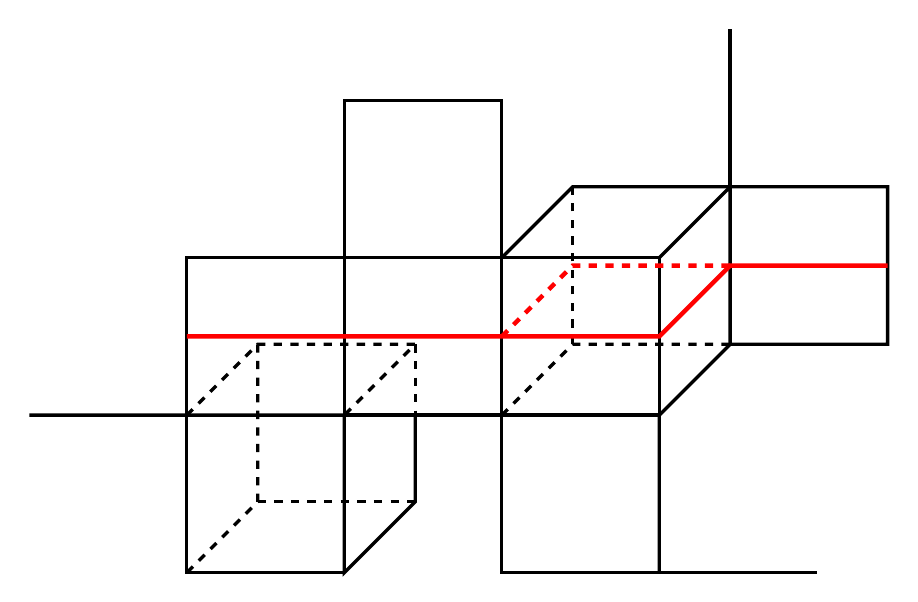
\begin{tikzpicture}[scale=2]
		\draw[very thick,dashed] (1,1) -- (1.45,1.45) -- (2.45,1.45) -- (2,1);
		\draw[very thick,dashed] (2.45,1.45) -- (2.45,1);
		\draw[very thick,dashed] (1.45,1.45) -- (1.45,.45) -- (1,0);
		\draw[very thick,dashed] (1.45,.45) -- (2.45,.45);
		\draw[very thick,dashed] (3,1) -- (3.45,1.45) -- (4.45,1.45);
		\draw[very thick,dashed] (3.45,1.45) -- (3.45,2.45);
		
		\draw[very thick] (0,1) -- (2,1) -- (2,0) -- (2.45,.45) -- (2.45,1);
		\draw[very thick] (2,0) -- (1,0) -- (1,2) -- (4,2) -- (4,1) -- (3,1) -- (3,3) -- (2,3) -- (2,0);
		\draw[very thick] (2,1) -- (3,1) -- (3,0) -- (5,0);
		\draw[very thick] (4,0) -- (4,1) -- (4.45,1.45) -- (5.45,1.45) -- (5.45,2.45) -- (3.45,2.45) -- (3,2);
		\draw[very thick] (4,2) -- (4.45,2.45) -- (4.45,1.45);
		\draw[very thick] (4.45,2.45) -- (4.45,3.45);
		
		\draw[ultra thick,color=red,dashed] (3,1.5) -- (3.45,1.95) -- (4.45,1.95);		
		\draw[ultra thick,color=red] (1,1.5) -- (4,1.5) -- (4.45,1.95) -- (5.45,1.95);
	\end{tikzpicture}

	\vfill
	{\Large Vorlesungsmitschrift von Phil Steinhorst} \\[.5cm]
	{\large Stand: \today}
	
\end{titlepage}
\cleardoubleemptypage